{\tabcolsep=17pt
\setlength\arrayrulewidth{1.5pt}
\newcommand\bhline{\arrayrulecolor{goldan-yellow}\hline\arrayrulecolor{black}}
\begin{longtable}[l]{!{\color{goldan-yellow}\vline width 1.5pt}rp{12cm}!{\color{goldan-yellow}\vline width 1.5pt}}
\bhline
\endfirsthead
\bhline
\endhead
\bhline
\endfoot
\endlastfoot
\raisebox{-3.2cm}{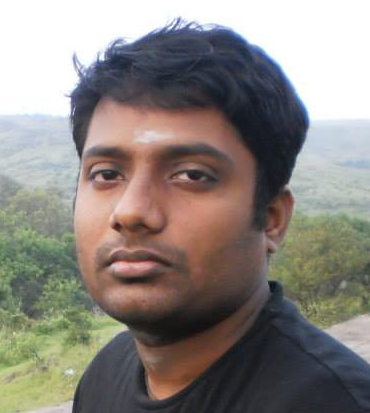
\includegraphics[scale=1.15]{src/Figures/authors/Balaji_Photo.jpeg}} & {\Large\bf S.B. Balaji}
\bigskip

\textit{S.B. Balaji received his B.E in Electronics and Communication Engineering from Madras Institute of Technology, Chennai, in 2008 and M.Tech from the Department of Electrical Engineering, Indian Institute of Technology, Kanpur in 2010 and Ph.D. from Department of Electrical Communication Engineering, Indian Institute of Science, Bengaluru, in 2018. His research interests include coding theory and information theory.}\\
 &\\[15pt]
\raisebox{-2.5cm}{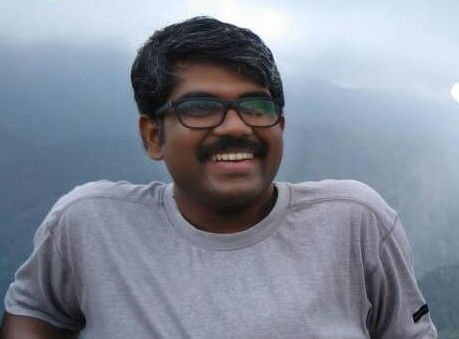
\includegraphics{src/Figures/authors/Biren.jpeg}} & {\Large\bf Birenjith Sasidharan}

\vskip .55cm


\textit{Birenjith Sasidharan received B.Tech. in Electronics and Communication Engineering from College of Engineering, Trivandrum and M.Sc. (Engg.) from Indian Institute of Science, Bengaluru in 2008. During 2008--2011, he was on the faculty of Electronics and Communication Engineering at Government Engineering College, Kannur in Kerala. In 2016, he completed his Ph.D. at the department of Electrical Communication Engineering in Indian Institute of Science, Bangalore. Since 2016, he has been working as Assistant Professor at Government Engineering College, Barton Hill at Thiruvananthapuram, Kerala. His research interests include code constructions for distributed storage.}\\
 &\\[15pt]
\raisebox{-3.2cm}{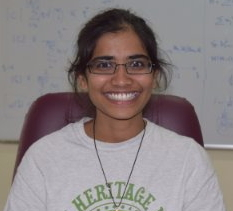
\includegraphics[scale=1.3]{src/Figures/authors/Myna_Vajha.jpeg}} & {\Large\bf Myna Vajha}

\vskip .55cm

\textit{Myna Vajha received B.Tech in Electronics and Electrical Communications Engineering from IIT Kharagpur in 2011, and Masters from EE Department, University of Southern California (USC), in 2013. She is currently a Ph.D. student at the department of Electrical Communication Engineering in Indian Institute of Science, Bengaluru. She has worked with Ericsson and Qualcomm in the past as a software architect, engineer respectively. Her research interests include coding theory and information theory, with applications to distributed storage systems.}\\
&\\[15pt]
\raisebox{-3.7cm}{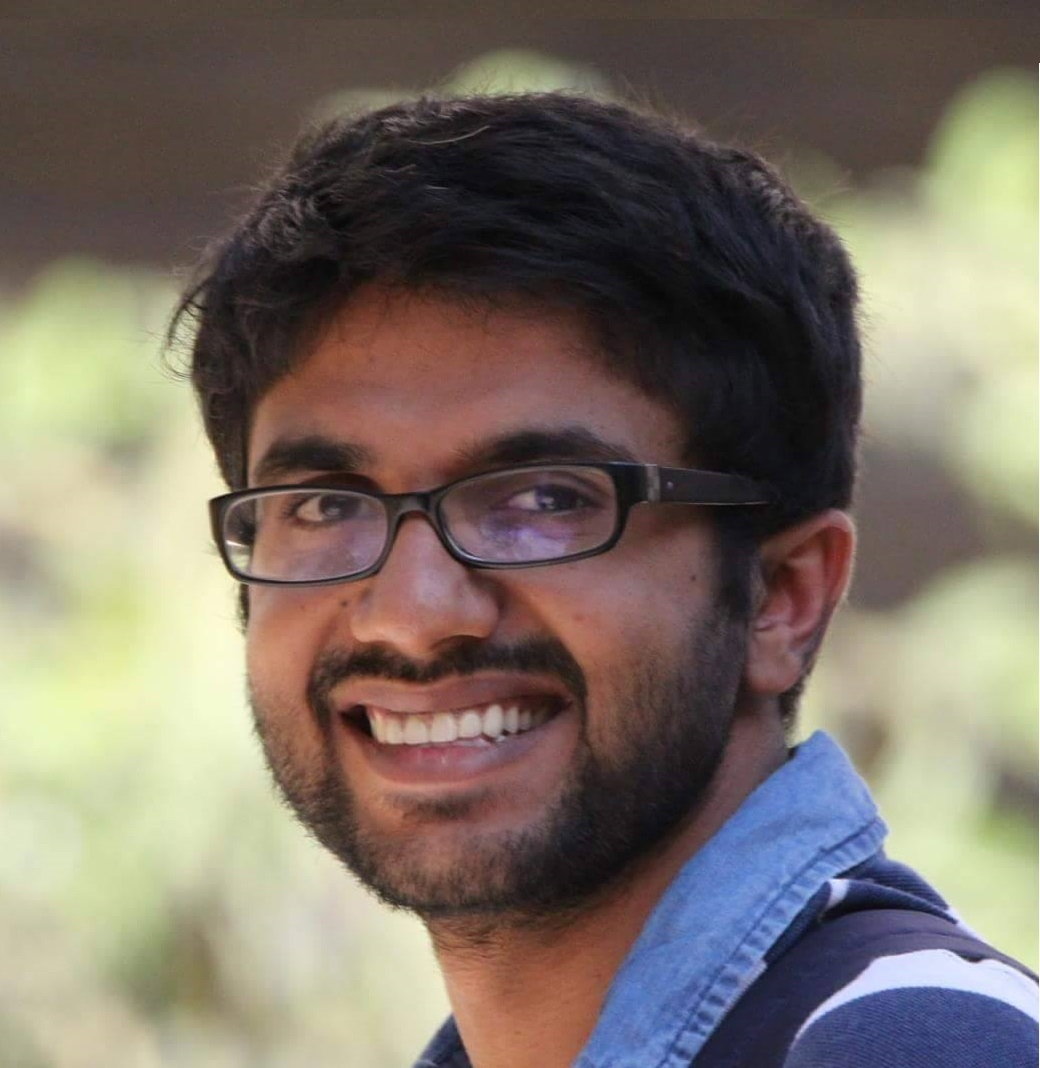
\includegraphics[scale=.44]{src/Figures/authors/Nikhil_photo.jpeg}} & {\Large\bf M. Nikhil Krishnan}

\vskip .55cm

\textit{M. Nikhil Krishnan received his B.Tech. in Electronics and Communication Engineering from Amrita School of Engineering, Kollam, in 2011 and M.E. in Telecommunication from the Indian Institute of Science (IISc), Bengaluru, in 2013. He is currently a Visvesvaraya Ph.D. scholar at the Department of Electrical Communication Engineering, IISc. His research interests include coding theory and information theory.}\\
&\\[7pt]
\raisebox{-4.2cm}{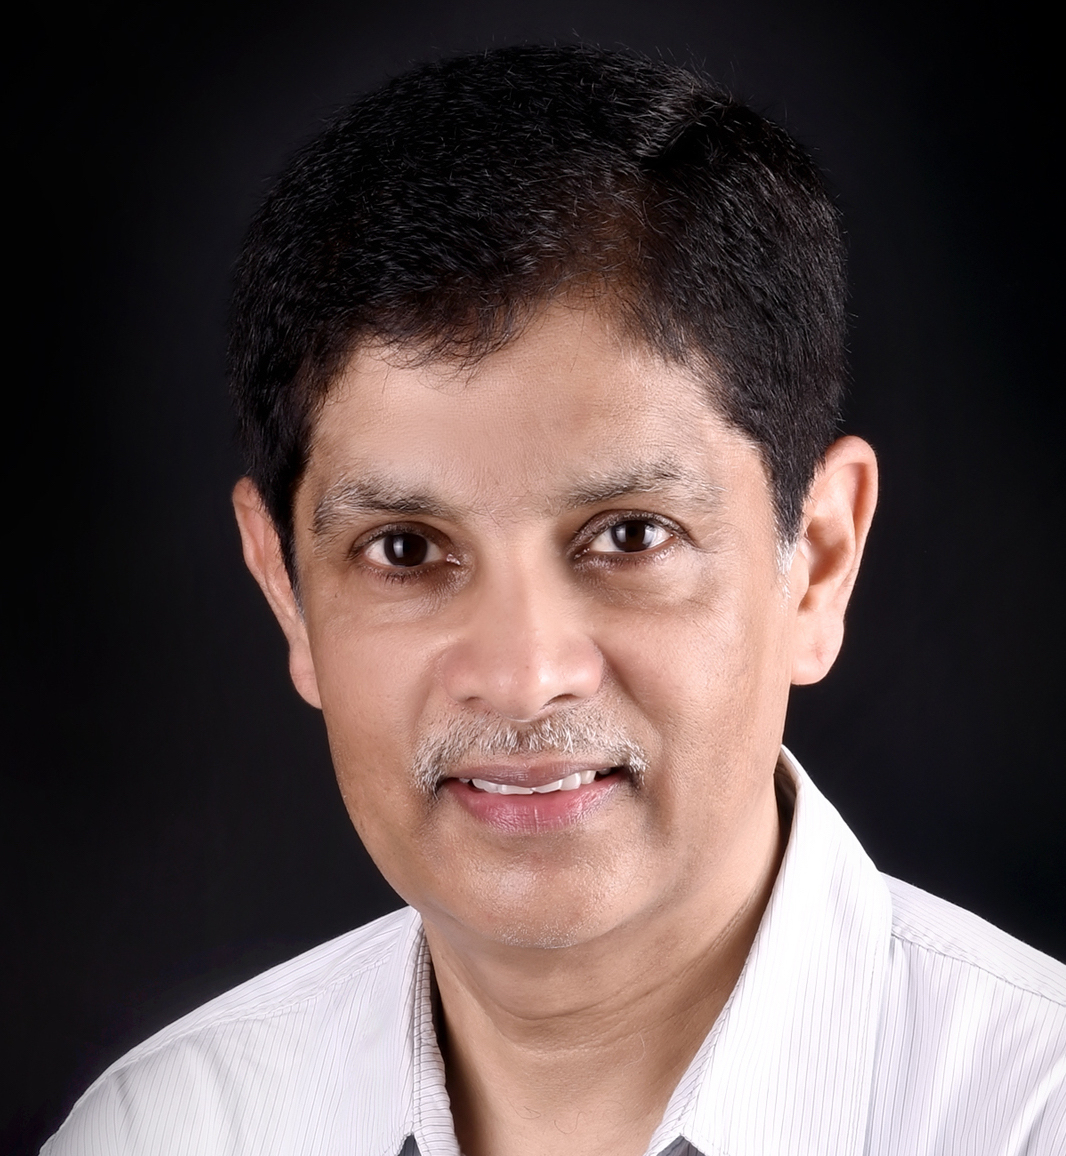
\includegraphics[scale=.83]{src/Figures/authors/PVK_ACCSJPG.jpeg}} & \raisebox{-1.1cm}{\Large\bf P. Vijay Kumar}

\vskip .55cm

\textit{P. Vijay Kumar received the B.Tech. and M.Tech. degrees from IIT Kharagpur and IIT Kanpur respectively, and the Ph.D. degree from USC in 1983, all in Electrical Engineering. From 1983 to 2003 he was on the faculty of the EE-Systems Department at USC. Since 2003, he has been on the faculty of IISc Bengaluru. He currently also holds the position of Visiting Professor at USC.}\\
 & \\
\multicolumn{2}{!{\color{goldan-yellow}\vline width 1.5pt}p{17.5cm}!{\color{goldan-yellow}\vline width 1.5pt}}{\textit{His research interests include codes for distributed storage and wireless communication. He is a recipient of the 1995 IEEE Information Theory Society Prize-Paper award and the IEEE Data Storage Best Paper Award of 2011/2012.  A pseudorandom sequence family designed in a 1996 paper co-authored by him now forms the short scrambling code of the 3G WCDMA cellular standard.   He received the USC School of Engineering's Senior Research Award in 1994, the Rustum Choksi Award for Excellence in Research in Engineering in 2013 at IISc and the 2017-22 J.C. Bose National Fellowship awarded by the Department of Science and Technology.  He was on the Board of Governors of the IEEE Information Theory Society in 2013-15, and 2019-21, was a plenary speaker at ISIT 2014 and a TPC Co-Chair of ISIT 2015.  He is a Fellow of the INAE, IAS and INSA Indian academies.}}\\
&\\[10pt]
\raisebox{-2.7cm}{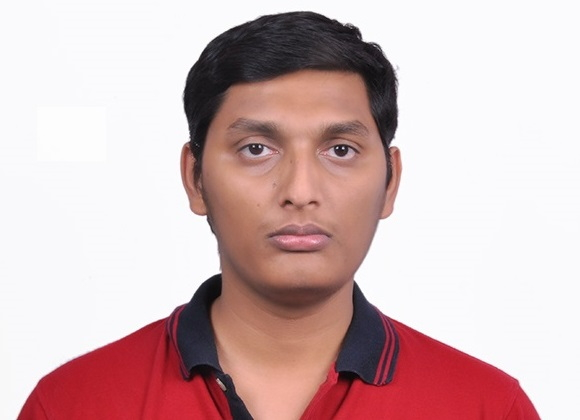
\includegraphics[scale=.9]{src/Figures/authors/Vinayak_photo.jpeg}} & {\Large\bf Vinayak Ramkumar}

\vskip .55cm

\textit{Vinayak Ramkumar received his B.Tech. in Electronics and Communication Engineering from National Institute of technology, Calicut, in 2015 and M.Sc. (Engg) from the Department of Electrical Communication Engineering, Indian Institute of Science (IISc), Bengaluru, in 2017. He is currently a Ph.D. student at the Department of Electrical Communication Engineering, IISc. His research interests include coding theory and information theory.}\\[10pt]
\bhline
\end{longtable}}\relax
